Anomalous isolated signals with energies that can exceed 100 GeV have been observed in the ECAL. These deposits, called "spikes", occur at a rate that is proportional to the collision rate. These "spikes" create issues for triggering at high luminosity and can cause large biases in the reconstructed energies and times of electrons, photons, jets, and in the computation of the missing transverse energy in an event. Spikes result from particles striking the APDs in the ECAL barrel directly and occasionally cause large anomalous signals through direct ionization of the silicon.\cite{Petyt:2012upa} Spikes predominately deposit energy in a single crystal and are characterized by a "spike" like pulse shape with a fast rise-time and no scintillation component. Typically there is little or no activity in the crystals surrounding the crystal in which the spike occurs, though occasionally a "double" spike does occur where spike-like signals are seen in two adjacent crystals. A rechit that is produced by a spike in a crystal will be referred to as a "spike rechit". The performance of traditional flags to reject spike rechits were studied when used with the CC algorithm. The rechit collections for both the ratio and the CC algorithms were produced and stored without any downstream cleaning, filtering, or calibration for this study. The CC reconstruction was preformed without OOT amplitude corrections to minimize the impact of the energy dependence on the time reconstruction. Such collections will be referred to as "raw" rechit collections.


% ... reject spike rechits were studied when used with the CC algorithm in runs 316241 - 316245 in the 2018A era. 
%-------------------------------- notes
%\textcolor{red}{ecal spikes are bvlaaa   ~cit a brief intro expand on spikes and why we are looking at them, comment on why the "spike" bump is not displaced as much as the ratio ( KUCC not sensitive to fast rise time of spike pulses ) }
\hfill
\begin{figure}[h!tbp]
\begin{center}
\resizebox{0.75\textwidth}{!}{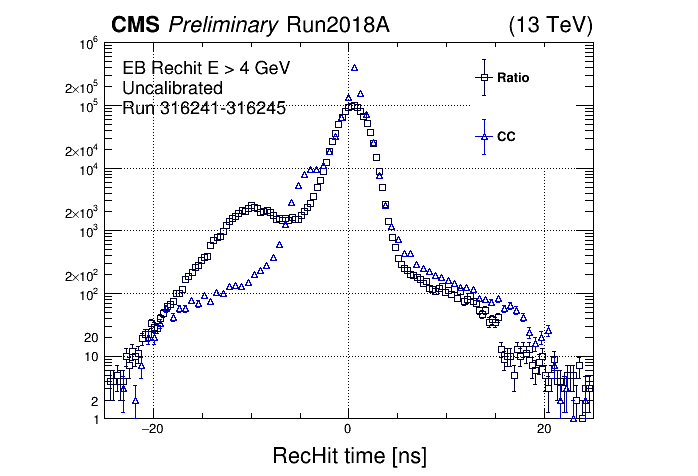
\includegraphics{fig/sec_gen/tr_hl_spike_distro_10062022142744.png}}
\caption{The distribution of the rechit times reconstructed using the ratio algorithm and the CC algorithm are plotted. The distributions were plotted for a rechits with energy $>4$ GeV. Full rechit collections are produced for both the ratio and CC reconstruction. These collections were saved as output by the producers without downstream cleaning, filtering, or calibrations. The bumps in the distributions located at roughly -10 ns in the distribution for the ratio method and -5 ns for the CC method correspond to spike rechits.}
%produced in runs 316241-316457 of Run 2018A and 
\label{raw_distro}
\end{center}
\end{figure}

In Figure~\ref{raw_distro} the distribution of the rechit times in the raw collections for both the CC and ratio method is shown for rechits in which the rechit energy is $>4$ GeV. The bumps located at roughly -10 ns in the distribution for the ratio method and -5 ns for the CC method correspond to rechits resulting from spikes. In Figure~\ref{2d_raw_distro_comp} the raw rechit times produced with the CC algorithm are plotted with respect to the raw rechit times produced with the ratio algorithm for rechits with energies between 10 GeV and 120 GeV. In this plot we can see that there is a strong correlation between the reconstructed times for the two methods. It can also be seen that the CC method produces a much narrower spread for prompt times than the ratio method. The "spike" rechit population is located between -6 ns and -15 ns on the ratio time axis and between -2 ns and -10 ns on the CC time axis.

\hfill
\begin{figure}[h!tbp]
\begin{center}
\resizebox{0.7\textwidth}{!}{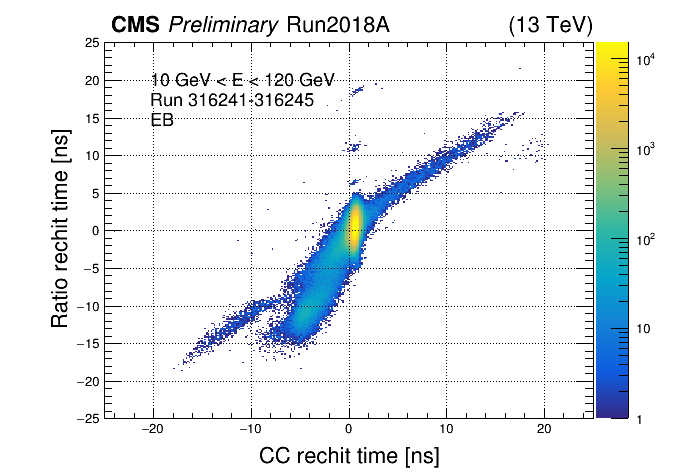
\includegraphics{fig/sec_gen/tr_2d_RtvCC_spike_10062022125336.png}}
\caption{The times for raw rechit collections for the CC algorithm and the ratio algorithm is plot with respect to each other for rechit energies between 10 GeV and 120 GeV. It can seen that there is a strong correlation between the reconstructed times for the two methods and that the CC method produces a much narrower spread for prompt times than the ratio method. The "spike" rechits found in the population located between -6 ns and -15 ns for ratio algorithm and between -2 ns and -10 ns for KUCC algorithm.}
\label{2d_raw_distro_comp}
\end{center}
\end{figure}

As was seen in Figure~\ref{raw_distro} and Figure~\ref{2d_raw_distro_comp}, it is characteristic of a spike rechit that the spike-like pulse shape results in a reconstruction with a time that is significantly earlier then for a non-spike rechit. The fast rise-time of the uncharacteristic shape of a spike signal causes the ratio algorithm to reconstruct a significantly earlier time for spike rechits. The CC algorithm is less sensitive to the bias introduced by the fast rise time and reconstructs a time that is less significantly early but still earlier than non-spike rechits. It is also characteristic of a spike rechit that they are isolated from other rechits. Since a crystal with a large energy deposition that is isolated from other crystals with activity is inconsistent with an electromagnetic shower, an isolated rechit would not be expected for non-spike rechits. A spike rechit can then be identified by looking at both the isolation of the rechit and the reconstructed time of the rechit.

\hfill
\begin{figure}[h!tbp]
\begin{center}
\resizebox{0.375\textwidth}{!}{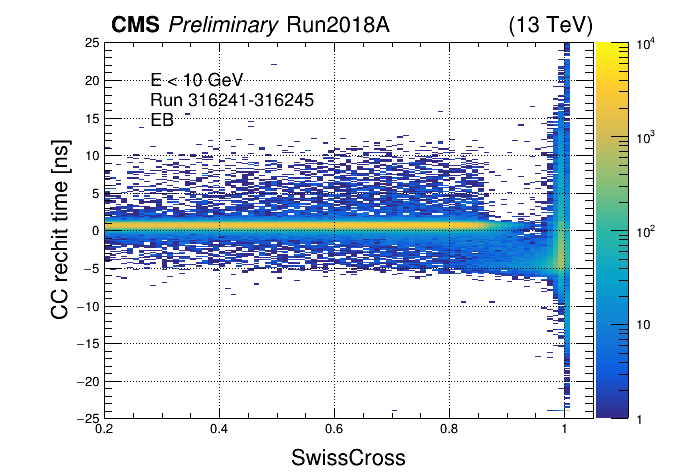
\includegraphics{fig/sec_gen/tr_2d_CC_swisscross1_10062022134628.png}}
\resizebox{0.375\textwidth}{!}{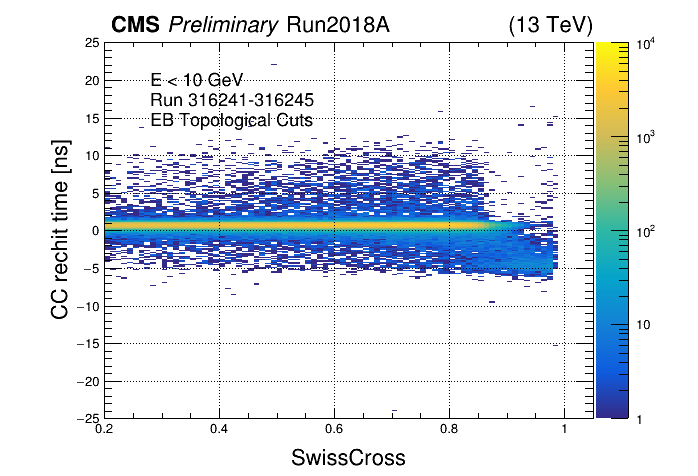
\includegraphics{fig/sec_gen/tr_2d_CC_swisscross2_10062022134846.png}}
\resizebox{0.375\textwidth}{!}{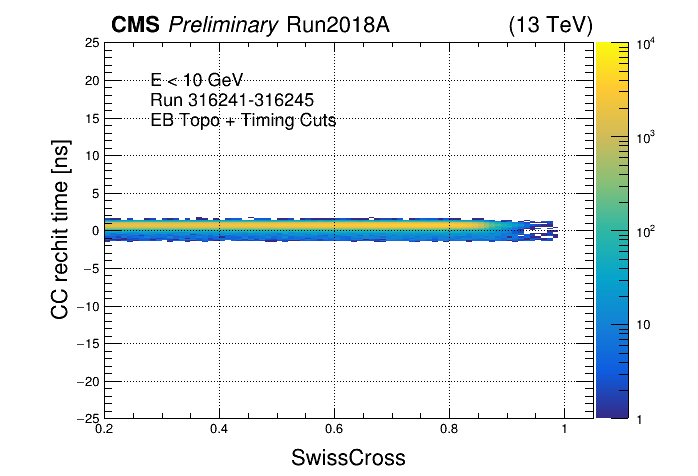
\includegraphics{fig/sec_gen/tr_2d_CC_swisscross3_10062022135015.png}}
\caption{Swiss-cross is plotted with respect to the CC reconstructed time for rechits with energy $>10$ GeV. In the plot on the top left the full distribution is shown with no spike flag cuts applied. As can be seen, this plot is composed of two populations, "non-spike" rechits spread around a time of 0 ns with a swiss-cross $>0.95$ and "spike" rechits spread around a swiss-cross of 1.0 with a "bump" located roughly at a time of -5.0 ns. In the plot on the right the topological flags are applied as cuts to reject spike rechits. With these cuts most of the "spike" rechits are rejected with the exception of "bump" located roughly at -5.0 ns. In the bottom plot the kOOT flag cut is also applied in addition to the topological cuts.  For the kOOT flag a value of 3 ns is used for all threshold parameters. Here it is seen that all "spike" rechits are rejected.}
\label{swisscross_CC}
\end{center}
\end{figure}

The swiss-cross variable characterizes the energy sharing between a crystal with a high energy signal and its neighboring crystals. The swiss-cross can be thought of as a ratio where the more isolated a rechit is the closer the swiss-cross value is to one. The swiss-cross is used to define two spike rechit rejection flags. The kWeird flag that rejects rejects rechits with isolated energy depositions, and the kDiWeird flag that is designed to reject double spikes.\cite{Petyt:2012upa} The use of the combination of kWierd or kDiWierd is refereed to as topological ( topo ) cuts. In the time reconstruction algorithm a spike rechit rejection flag called kOutOfTime ( kOOT ) is defined based on energy dependent time thresholds that can be set independently for the barrel, the endcaps, and both the high and low energy reconstruction regions. This threshold defines a "window" around the "prompt" times and flags any times that fall outside this window in both the early and delayed sides of the time distribution. 
%While parameters exist to set the thresholds separately for "early" and "delayed" sides of the time distribution, they are traditionally set to the same values.

In Figure~\ref{swisscross_CC} the swiss-cross is plotted with respect to the CC reconstructed time for rechits with energy $>10$ GeV. In the plot on the top left the full distribution with no spike rechit cuts applied. As can be seen, this plot is composed of two populations, "non-spike" rechits spread around a time of 0 ns with a swiss-cross $>0.95$ and "spike" rechits spread around a swiss-cross of 1.0 with a "bump" located roughly at a time of -5.0 ns. In the plot on the right, the topological cuts are applied. With these cuts most of the "spike" rechits are rejected with the exception of "bump" located roughly at -5.0 ns. In the bottom plot the kOOT flag is applied in addition to the topological cuts. In this plot a threshold value of 3 ns is used for all kOOT threshold parameters as is the default in the ratio algorithm. In this plot it can be seen that the majority of "spike like" rechits are rejected.

If a rechit is flagged as kOOT, that rechit is much less likely to be utilized in down stream particle reconstruction and thereby impacting the energy of these reconstructed particles.  In order to avoid adverse impact on the energies of the reconstructed particles it was necessary to carefully tune the thresholds used to set the kOOT flag with the CC time reconstruction. Since times reconstructed with the CC algorithm depends on the amplitudes it a significantly different manner then the ratio reconstruction, the thresholds for low and high energies tuned independently.  Appropriate thresholds where determined in order to maximize spike rechit rejection, as seen in Figure~\ref{swisscross_CC} , without negatively impacting the down stream particle reconstruction, across all reconstructed rechit energies.

%it was necessary to separately tune the thresholds for low and high energies.  Several studies were conducted to fine tune the kOOT threshold parameters in order to maximize spike rechit rejection without negatively impacting the down stream particle reconstruction across all reconstructed rechit energies.   

%To fully characterize the performance of the spike rechit rejection flags, a spike rechit rejection "efficiency" is defined and plotted with respect to the rechit energy. In order to do this a criteria to select "spike" rechits is needed. A rechit is defined as "isSpike" if its swiss-cross is $>0.95$. With this a "Spike" rechit rejection "efficiency" ($\epsilon_{Spike}$) is defined in Equation~\ref{spike_eff}.

% \rm{} removes itailics   or \mathrm{}   \texttt{}  and texgt scaling set font size
% define a symbol  and use logic symbols
%\begin{equation}\label{spike_eff}
%\epsilon_{Spike}= \frac{\mathrm{isSpike\,\&\&\,}(\mathrm{kWeird\,||\,kDiWeird\, ||\,kOOT})}{\mathrm{isSpike}}\quad
%\end{equation}

%In Figure~\ref{spike_reject} $\epsilon_{Spike}$ is plotted with respect to the rechit energy for both the ratio and KUCC method, where the kOOT flag is produced using the default ratio values, for rechits with an energy $>4$ GeV. At rechit energies $>~30$ GeV the $\epsilon_{Spike}$ for both KUCC and ratio methods approaches 100\%. For energies $<~30$ GeV, $\epsilon_{Spike}$ for the KUCC method closely aligns with the $\epsilon_{Spike}$ seen for the ratio method. It is important to note that the "isSpike" criteria is a loose selection for spike-like rechits and that $\epsilon_{Spike}$ is dependent on the kOOT flag production parameters chosen.

%\hfill
%\begin{figure}[h!tbp]
%\begin{center}
%\resizebox{0.7\textwidth}{!}{\includegraphics{fig/sec_gen/swisscross_CC_topo.png}}
%\caption{caption needed 
%\textcolor{red}{? place holder ?}
%}
%\label{swisscross_CC_topo}
%\end{center}
%\end{figure}

%\hfill
%\begin{figure}[h!tbp]
%\begin{center}
%\resizebox{0.7\textwidth}{!}{\includegraphics{fig/sec_gen/swisscross_CC_time.png}}
%\caption{caption needed 
%\textcolor{red}{? place holder ?}
%}
%\label{swisscross_CC_time}
%\end{center}
%\end{figure}

%\hfill
%\begin{figure}[h!tbp]
%\begin{center}
%\resizebox{0.7\textwidth}{!}{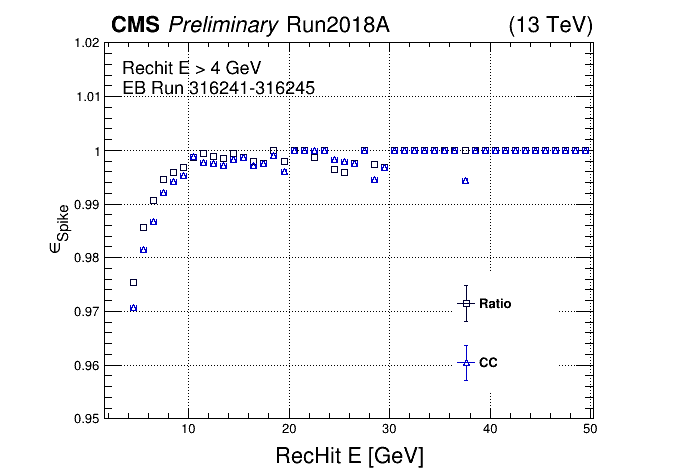
\includegraphics{fig/sec_gen/tr_hl_spike_eff_10062022141907.png}}
%\caption{$\epsilon_{Spike}$ is plotted with respect to the rechit energy for both the ratio and KUCC method for rechits with an energy $>4$ GeV. At rechit energies $>~30$ GeV the $\epsilon_{Spike}$ for both KUCC and ratio methods approaches 100\%. For energies $<~30$ GeV, $\epsilon_{Spike}$ is very close to that shown by the ratio method but slightly degraded with the threshold value used to set the kOOT flag.}
%\label{spike_reject}
%\end{center}
%\end{figure}

%The threshold parameters to be utilized to set the kOOT flag in KUCC algorithm were determined by studying the dependence of $\epsilon_{Spike}$ with respect to the "notSpike" RH rejection "effeciency" ($\epsilon_{notSpike}$) as defined in Equation~\ref{notspike_eff} in a "ROC" style plot.

%\begin{equation}\label{notspike_eff}
%\epsilon_{notSpike}= \frac{\mathrm{!\,isSpike\,\&\&\,}(\mathrm{kWeird\,||\,kDiWeird\, ||\,kOOT})}{\mathrm{!\,isSpike}}\quad
%\end{equation}

%In this plot, shown in Figure~\ref{spikr_reject_roc}, it is important to note that these values do not correspond to any "truth labeled" data and is only used for performance comparisons in order to make an informed decisions when selecting threshold parameters. As can be seen in this plot, a number of thresholds were studied for the KUCC method (green triangles) including both symmetric thresholds where the parameters for the early and delayed sides of the distribution are set the same value, and asymmetric thresholds where a different value for the two parameters is set. For reference the data point for the ratio method with the default symmetric threshold at 5 ns is shown (black inverted triangle). It was determined that a symmetrical threshold parameterization that erred on the side of a better $\epsilon_{Spike}$ was preferable. Given this criteria there kOOT parameters for the KUCC method are set to 2.25 ns. This selection gives a $\epsilon_{Spike}$ of $\sim$0.985\% and a $\epsilon_{notSpike}$ of $\sim$0.025\%. the same parameters as determined for EB are also used for the EE parameters.

%\hfill
%\begin{figure}[h!tbp]
%\begin{center}
%\resizebox{0.7\textwidth}{!}{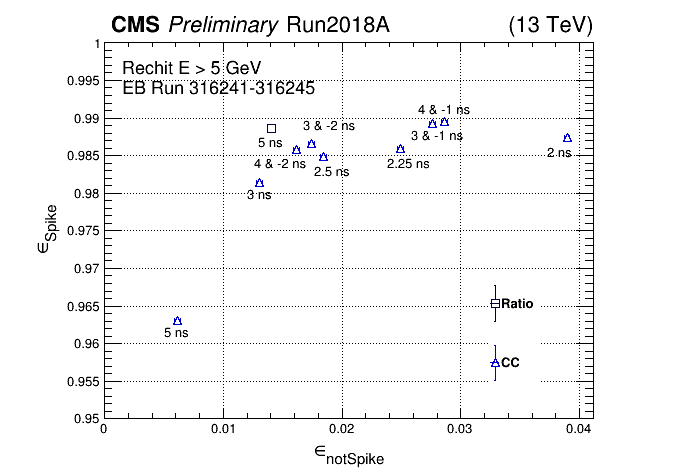
\includegraphics{fig/sec_gen/tr_hl_spike_roc_22062022103006.png}}
%\caption{$\epsilon_{Spike}$ is plotted with respect to $\epsilon_{notSpike}$ for different parameter settings for the kOOT flag produced for the KUCC method (blue triangles) including both symmetric thresholds where the parameters for the early and delayed sides of the distribution are set the same value, and asymmetric thresholds where a different value for the two parameters is set. For reference the data point for the ratio method with the default symmetric threshold at 5 ns is shown (black square). It is important to not that these values do not correspond to any "truth labeled" data.}
%\label{spikr_reject_roc}
%\end{center}
%\end{figure}